%************************************************
\chapter{Structural Aspects}\label{ch:structural_aspects}
%************************************************

Subjecting the anisotropic network model to a critical
examination of its structural features, we identify prevalent
patterns of connectivity and relate theoretical and computational
results to findings from experiments in the rat's cortex.


\section{Introduction}

Investigation \marginpar{
  \begin{center}
    
\includegraphics[width=0.9\linewidth]{img/HCP_text_logo.png}
  \end{center} \vspace{-0.3cm}
  \mbox{\textrm{\href{http://www.humanconnectome.org/}{humanconnectome.org}}}}
of the brain's connectivity is an ongoing endeavour.  Concurrent
collaborative efforts like the Human Connectome Project, the Open
Connectome Project and the Allen Brain Atlas, intent on mapping the
'wiring' of the brain, as well as the continued development of
experimental techniques and computational resources, demonstrate
\marginpar{Open Connectome Project
  \href{http://www.openconnectomeproject.org/}{openconnectomeproject.org}}the
great interest in advancing this field.

Research in brain connectivity spreads over the whole scale
% ---------------------------------------
\marginpar{%
  \begin{center}
    
\includegraphics[width=1.\linewidth]{%
      img/AllenBrainLogo.png}
  \end{center}\vspace{-0.3cm}%
  \mbox{\textrm{\href{http://www.brain-map.org/}{brain-map.org}}}%
  }
% ---------------------------------------
of the brain; from the mapping of fiber pathways between brain regions
at the macroscopic level, to the synaptic connections of individual
neurons on the microscale, researchers are trying to identify the
links that enable the brain its characteristic cognitive abilities.
%Macroscale: Can cite Sporns2004 In the search for structural
connections, these links are of anatomical nature. However,
statistical dependencies and causal relationships between the distinct
computational units in the brain are being researched with equal
emphasis \parencite{Scholarpedia-BrainConnectivity}. Connectivity in
the context of the anisotropic network model introduced in
Section~\ref{sec:anisotropic_network_model}, refers in this chapter to
structural links. So far, we have only briefly mentioned that the
network's nodes should be interpreted as individual neurons; to allow
for a discussion of functional relationships between nodes, we have
yet to provided a physical description of a neuron's function. Here we
explore the network's structural connectivity, modeling synaptic
contacts between axon and dendrites of individual neurons.




In the local cortical circuits the anisotropic geometric model was
\marginpar{synaptic connectivity} derived from, synaptic connectivity
is a major mode of configuration.  In those networks, connectivity has
been determined to be neither completely random nor exclusively
specific; recurring patterns of connectivity have been identified by
several reports \parencite{Sporns2004,Song2005,Perin2011}.

The impact of this structural specifity discovered in local networks
is shown to be significant; while linking network structure to network
dynamics remains an active field of research, several studies were
able to employ computational and theoretical models to establish such
a connection. A study by \textcite{Zhao2011}, for example,
demonstrates how second order connectivity statistics affect a
network's propensity to synchronize. In the same year, Alex Roxin
reported on the influence of in- and out-degree distributions on
dynamics of neural network \parencite{Roxin2011}. Later,
Pernice et al. were able to link structural connectivity to spike
train correlations in neural networks
\parencite{Pernice2011}.

Experimentally, paired intracellular recordings are used to
\marginpar{mapping synaptic connectivity in experiments} determine
synaptic connectivity in cortical slices. Using two electrodes, one
inserted in the cell and one outside the cell, a single intracellular
recording allows for measurement of a cell's membrane potential
\parencites[Chapter 3]{Brette_Neural-activity}[]{Scholarpedia-IntracellularRecording}. Simultaneous
recordings from multiple neurons are then able to infer synaptic
connectivity by evoking an action potential through current injection
in one neuron and observing the change of membrane potential in the
other cells \parencite{Song2005}.

%\vspace{0.35cm}
\begin{figure}[H]
  \centering
  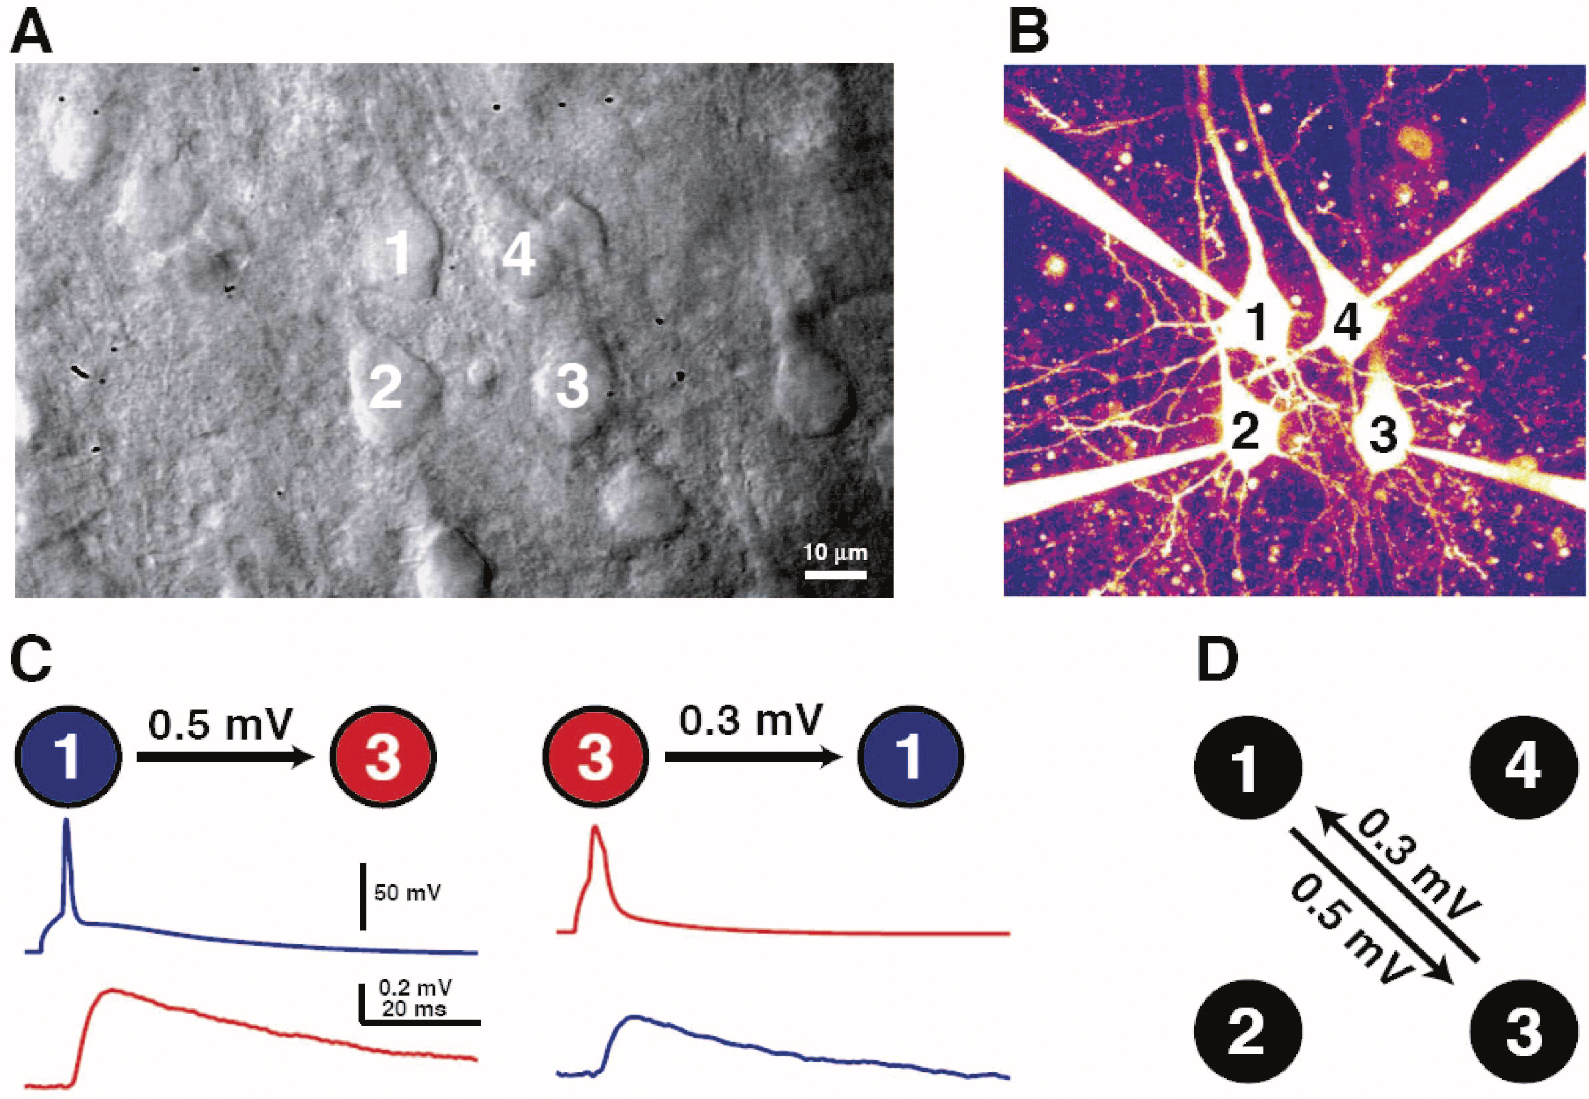
\includegraphics[width=.75\linewidth]{img/song2005-quadruplet_recordings.png}
  \caption{Song et al. use quadruple whole-cell recordings, observing
    simultaneously the membrane potential of four neurons.
    \textbf{A)} Contrast image showing four thick-tufted L5 neurons
    \textbf{B)} Fluorescent image of the same cells after patching on
    \textbf{C)} Evoking an action potential in the presynaptic neuron
    causes characteristic membrane potential change in the
    postsynaptic neuron \textbf{D)} Infering synaptic connectivity
    from the EPSP waveform observed in C). Image from \textcite{Song2005}.
    % \texttt{\textcolor{linkgrey}{3b056efe-3ebc}}
  }
\end{figure}
%\vspace{0.45cm}

While techniques for paired intracellular recordings are rapidly
developing, their ability to capture connectivity patterns of large
networks is yet very limited. To this date, the connectome of
\textit{C. Elegans} remains the outstanding exception of a
connectivity configuration that has been fully mapped
\parencite{White1986}. Even in the state-of-the-art experiment
conducted by Perin et al., using a setup capable of recording up to
twelve neurons simultaneously, the authors note that an investigation
of degree distribution was not carried out, due to lack of sufficient
data
\parencite{Perin2011}.

Working with a geometrical network model and its computational
\marginpar{exploiting the benefits of a geometrical model}
implementation, such restrictions disappear; the full information
about the network, in form of its connectivity matrix, is given at
point in time and can be easily queried for. Experiments that may take
days to perform \textit{in vivo}, can be completed in a matter of
seconds \textit{in silico}. As such, geometrical models lend
themselves to extensive examination of their structural aspects.  In
trying to exploit these advantages, two approaches present
themselves. One may construct a network model that extrapolates the
known biological configuration; a full structural examination of these
networks could possibly expose relevant patterns not yet observed. For
this approach a sophisticated understanding of the biological
configuration is critical. Neuron morphology, however, is difficult to
describe and extract. For this analysis we suggest a reductionist
approach. Having motivated an abstract model reflecting a cortical
network's anisotropy in connectivity, we distinguish emerging
structural patterns, specific to anisotropic networks, from results,
that only indirectly stem from the network's anisotropy, in the hopes
to be able to characterize the significance of directional
heterogeneity in structural connectivity of cortical circuits.


In this chapter we subject the anisotropic network model introduced in
Section~\ref{sec:anisotropic_network_model} to a critical analysis of
its structural aspects. General network topology, as well as specific
modes and patterns of connectivity, are to be identified and laid out
for comparison with findings in biological neural networks.  In an
effort to identify structural features that can be directly associated
with the network's anisotropy in connectivity, \marginpar{rewired and
  \mbox{distance-depen}\-dent networks as reference} it is crucial to
differentiate such findings from results that are only indirectly
caused by the network's anisotropy. To this end we are recruiting the
different network types introduced in the previous chapter throughout
this analysis. Having shown a decreasing degree of anisotropy in
rewired and distance-dependent networks, both models will serve as
reference to compare against for structural features found in
anisotropic networks. Analyzing standard graph measures in the first
two sections, we quickly move on to towards neuronal network specific
connectivity and anisotropy's role in being able to model such highly
non-random patterns in the later sections.


% ######################################################################### %
% ------------------------------------------------------------------------- %
%                             Comment Stuff
% ------------------------------------------------------------------------- %
% ######################################################################### %


% Human Connectome Project and the Open Connectome Project, the
% continued development of experimental techniques and of resources
% like the Brain Connectivity Toolbox software, as well as the
% research of theoreticians and experimentalists, are all dedicated
% towards the common goal of charting brain connectivity.

% In this general sense, brain connectivity can refer to linking
% between distinct units at various scales. From the mapping of fiber
% pathways between brain regions on the macroscale, to the synaptic
% connections of individual neurons on the microscale,
% [\textcolor{linkgrey}{Scholarpedia}].

% It is interesting not only to investigate for anatomical
% connections, but functional and causal as well. However, exploring
% the aspects of our specific geometric network model, in this chapter
% the connectivity of interest to us is the structural connectivity at
% the microscale, that is synaptic connections between individual
% neurons.

% \marginpar{Human Connectome Project
% \mbox{\url{humanconnectome.org}}}

% \parbox{1.8cm}{Human Connectome
% Project}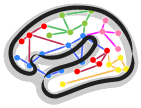
\includegraphics[width=0.45\linewidth]{img/HCP_logo.png}
% \mbox{\url{humanconnectome.org}}}


% Ho Ko connectivity -> specific dynamics.
% Pernice -> Spike Train Correlations. Maybe Shepherd 2005?

% ...and have been linked to brain function and dynamics.

% *What cool things synaptic connectivity does.  , stores memory, drives
% dynamics, etc.  While brain is plastic, there is structure that is
% believed to provide a framework, boundary conditions to

% *patterns of synaptic connectivity is neither completely random nor
% exclusively specific, patterns emerge [Sporns, Perin, Song]
 
% This specific, non-random connectivity largely impact dynamics and
% brain function:


% Connectivity in the directionally heterogenous geometric networks
% introduced in ??, models synaptic contacts between axon and
% dendrites of individual neurons. In this chapter

% It is then the task of this theoretical framework to provide results
% interesting to the biological situation. An investigation on how well
% an introduced model can reproduce certain structural aspects of
% networks that have already been fund is integral to the study of a
% computational model. But, furthermore, a model should aspire to
% extrapolate results found in the biological
% situation.



%%% Local Variables: 
%%% mode: latex
%%% TeX-master: "../dplths_document"
%%% End: 

\newpage

% ######################################################################### %
% ------------------------------------------------------------------------- %
%                     Degree distribution
% ------------------------------------------------------------------------- %
% ######################################################################### %

\section{Degree Distribution}\label{sec:degree_distribution}


The in- and out-degree of a vertex in a directed graph describes the
number of incoming and outgoing connection from and to other
\marginpar{cf. Definition~\ref{def:in_out_degree}} vertices. As a
fundamental concept in graph and network theory, the degree
distribution is integral in the categorization of networks and allows
for the estimation of graph properties. 

Node degree distribution was shown to have strong impact on the
dynamics of neuronal networks models commonly used in computational
neuroscience research \parencite{Roxin2011, Pernice2013}. Increasing
in-degree variance for example could be connected to the appearance of
oscillations in the network. Extracting degree distributions from
biological networks however, remains a challenge as many neurons need
to be tracked simultaneously to obtain enough data to confidently
estimate degree distributions.

\begin{figure}[H]
  \centering
  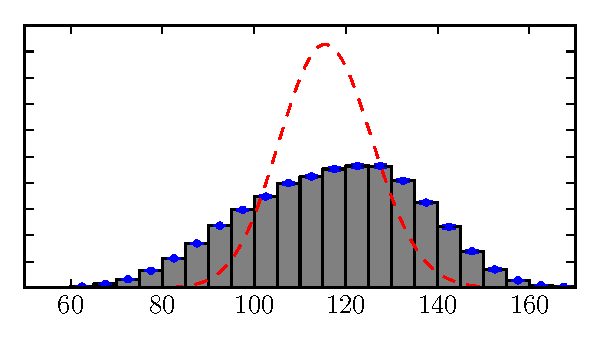
\includegraphics[width=0.65\textwidth]{%
    plots/9326138e.pdf}
  \caption{\textbf{In-degree distribution in anisotropic networks
      shows comparably high variance and is skewed to the left} From 250
    anisotropic networks in-degree distributions were extracted and
    are shown in a normed histogram plot, errorbars SEM. Comparison with the
    binomial degree distribution (red) of a Gilbert random graph model
    with matching parameter set ($N=1000$, $p =0.116$) shows higher
    variance of in-degrees in anisotropic networks (sample variance $=
    344.54$, variance of binomial distribution $Np(1-p) = 102.44$.)
    Skewness to the left of the sample is $-0.1763.$
    (\smtcite{9326138e})}
  \label{fig:in_degree_ER_compare}
\end{figure}

Here we analyze in- and out-degrees in the anisotropic network
model. First we find that compared to the binomial in-degree
distribution of a Gilbert random graph model, in-degrees of vertices
in anisotropic networks display higher variance and their distribution
is skewed to the left (\autoref{fig:in_degree_ER_compare}). However,
this specific in-degree profile is not an intrinsic property of
anisotropy, as the distribution remains stable under manipulation of
the anisotropy degree and closely matches the profile of a purely
distance-dependent network (\autoref{fig:in_degree_rewiring}). This
result agrees with findings of \textcite[Fig. S3]{Perin2011}, who were
able to recreate degree distributions from their experiment with layer
5 thick-tufted pyramidal cells in neonatal rats from the extracted
distance-dependent connection profiles alone.

\begin{figure}[H]
  \centering
  \renewcommand{\tabcolsep}{2pt}
  \setlength\extrarowheight{0pt}
  \begin{tabular}{lll}
    \begin{overpic}[width=0.28\textwidth]{%
        plots/77995b6b_in000.pdf}
      \put(12,56){\small $\eta = 0$}
    \end{overpic}
    &
    \begin{overpic}[width=0.28\textwidth]{%
        plots/77995b6b_in025.pdf}
      \put(12,56){\small $\eta = 0.25$}
    \end{overpic}
    &
    \begin{overpic}[width=0.28\textwidth]{%
        plots/77995b6b_in050.pdf}
      \put(12,56){\small $\eta = 0.5$}
    \end{overpic}
    \\
    \begin{overpic}[width=0.28\textwidth]{%
        plots/77995b6b_in075.pdf}
      \put(12,56){\small $\eta = 0.75$}
      \put(4,-4){\small$0$}\put(78,-4){\small$200$}
    \end{overpic}
    &
    \begin{overpic}[width=0.28\textwidth]{%
        plots/77995b6b_in100.pdf}
      \put(12,56){\small $\eta = 1$}
      \put(4,-4){\small$0$}\put(78,-4){\small$200$}
    \end{overpic}
    & 
    \begin{overpic}[width=0.28\textwidth]{%
        plots/77995b6b_indst.pdf}
      \put(12,56){\small distance}
      \put(4,-4){\small$0$}\put(78,-4){\small$200$}
    \end{overpic}
    \\
  \end{tabular}
  \caption{\textbf{In-degree distribution not affected by varying
      degrees of anisotropy} In-degree distributions from the 25
    sample graphs and their rewiring stages are plotted in normed
    histograms and listed from rewiring factor $\eta =0$ (original
    anisotropic) to $\eta = 1$ (completely rewired, maximal
    isotropy). Comparison shows that varying degrees of anisotropy do
    not influence the degree distribution, in fact in-degree
    distributions match with the degree distribution of an equivalent
    distance-dependent network shown bottom-right
    (\smtcite{77995b6b}). }
  \label{fig:in_degree_rewiring}
\end{figure}


While the out-degree distribution of vertices in the anisotropic
network also shows itself stable under rewiring, its distribution is
drastically different from the out-degree distribution in a comparable
distance-dependent network (\autoref{fig:out_degree_rewiring}). The
asymmetric, long-tailed distribution is identified as an artifact of
the anisotropic network's spatial confinement; a neuron, closely
located near a surface edge, might have an axon projection out of the
square causing minimal out-degree or, projecting through the entire
length of the surface, may have maximal out-degree. Approximating the
expected number of outgoing connections for a vertex in an anisotropic
network of size $N$, side-length $s$ and axon width $w$ as
\[
  N \frac{w l}{s^2},
\]
with parameters $N = 1000$ and $\frac{w}{s} = 0.252$, we obtain an
upper bound for the expected out-degree, 
\[
  N \frac{w l}{s^2} \leq N\frac{w}{s} \sqrt{2} \approx 350.
\]
If $f(l)$ is the probability density function to find axon length $l$
for a random node $v$ in the anisotropic network model, the out-degree
distribution is then approximated by
%
\begin{align}\label{eq:axon_length_approx}
  \mathbf{P}(d_{\mathrm{out}}(v) = N \frac{w l}{s^2}) = f(l),  
\end{align}
%
see also \autoref{fig:out_degree_ER_compare}.

\begin{figure}[H]
  \centering
  \renewcommand{\tabcolsep}{2pt}
  \setlength\extrarowheight{0pt}
  \begin{tabular}{lll}
    \begin{overpic}[width=0.28\textwidth]{%
        plots/77995b6b_out000.pdf}
      \put(12,56){\small $\eta = 0$}
    \end{overpic}
    &
    \begin{overpic}[width=0.28\textwidth]{%
        plots/77995b6b_out025.pdf}
      \put(12,56){\small $\eta = 0.25$}
    \end{overpic}
    &
    \begin{overpic}[width=0.28\textwidth]{%
        plots/77995b6b_out050.pdf}
      \put(12,56){\small $\eta = 0.5$}
    \end{overpic}
    \\
    \begin{overpic}[width=0.28\textwidth]{%
        plots/77995b6b_out075.pdf}
      \put(12,56){\small $\eta = 0.75$}
      \put(4,-4){\small$0$}\put(78,-4){\small$350$}
    \end{overpic}
    &
    \begin{overpic}[width=0.28\textwidth]{%
        plots/77995b6b_out100.pdf}
      \put(12,56){\small $\eta = 1$}
      \put(4,-4){\small$0$}\put(78,-4){\small$350$}
    \end{overpic}
    & 
    \begin{overpic}[width=0.28\textwidth]{%
        plots/77995b6b_outdst.pdf}
      \put(52,56){\small distance}
      \put(4,-4){\small$0$}\put(78,-4){\small$350$}
    \end{overpic}
    \\
  \end{tabular}
  \caption{\textbf{Out-degree distribution not affected by varying
      anisotropy but highly different from distance-dependent
      networks} Out-degree distributions from the 25 sample graphs and
    their rewiring stages are plotted in normed histograms and listed
    from rewiring factor $\eta =0$ (original anisotropic) to $\eta =
    1$ (completely rewired, maximal isotropy). While varying degrees
    of anisotropy do not influence the degree distribution, the
    characteristic out-degree profile is drastically different from
    the distribution found in equivalent distance-dependent networks
    (\smtcite{77995b6b}). }
  \label{fig:out_degree_rewiring}
\end{figure}


%------------------------------------------------
\marginpar{\vspace{1.91cm}\\Steep incline for small out-degree cut off
  due to binning (cf. \autoref{suppfig:out_degree})} 
%------------------------------------------------
\begin{figure}[H]
  \centering
  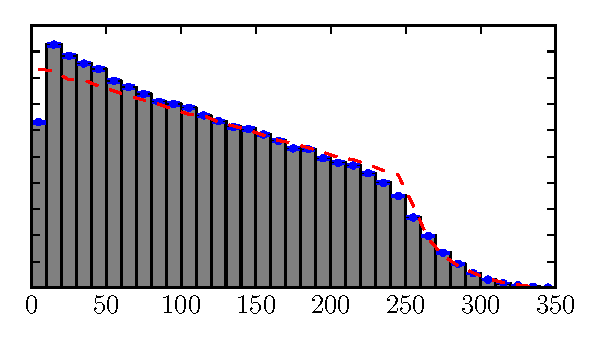
\includegraphics[width=0.65\textwidth]{%
    plots/019555b0.pdf}
  \caption{\textbf{Characteristic out-degree distribution as an
      artifact of network's boundaries} From 250 anisotropic networks
    out-degree distributions were extracted and are shown in a normed
    histogram plot, errorbars SEM. The characteristic distribution is
    identified as an artifact of the network's spatial confinement;
    using equation~\ref{eq:axon_length_approx} the out-degree profile
    is approximated (red) by the distribution of axon lengths in the
    anisotropic network (\smtcite{019555b0}).}
  \label{fig:out_degree_ER_compare}
\end{figure}



%%% Local Variables: 
%%% mode: latex
%%% TeX-master: "../dplths_document"
%%% End: 


% ######################################################################### %
% ------------------------------------------------------------------------- %
%                        Small World Properties
% ------------------------------------------------------------------------- %
% ######################################################################### %


\section{Small World Properties}\label{sec:small_world}

Sporns papers


%%% Local Variables: 
%%% mode: latex
%%% TeX-master: "../dplths_document"
%%% End: 


\section{Two Neuron Connections}

Connectivity in cortical neural networks shows a specific . First
described by Markram 1997, finding across have confirmed . 

A first result


\begin{figure}[htp]
  \centering
  \makebox{%
    \begin{overpic}[height=0.17\textheight]{%
        plots/c5f1462b_aniso_rand.pdf}
      %\put(89.8,56.5){\small\textbf{A}}
      %\put(14.3,78.9){\small\textbf{A}}
    \end{overpic}
    \hspace{0.45cm}
    \begin{overpic}[height=0.17\textheight]{%
        plots/c5f1462b_aniso_rew.pdf}      
       %\put(16.2,78.9){\small\textbf{B}}
      %\put(12,5){\small\textbf{B}}
    \end{overpic}
  }%
  \vspace{0.2cm}
  \caption{\textbf{Title} SEM!  (\smtcite{c5f1462b}).} %?? fix width issue!!
  \label{fig:two_neuron_probs}
\end{figure}  


%%% Local Variables: 
%%% mode: latex
%%% TeX-master: "../dplths_document"
%%% End: 

 
\section{Tuning distance-dependency}

Stepping away, we 




Maybe simplicity of the model makes stuff wrong. Tune to Perin
distance profile.

Let 

In their study, \textcite{Perin2011} heavily rely on a
distance-dependent 


Here we introduce anisotropic networks tuned to reflect a given
distance-dependent connection profile. We face the following: Given
$C(x):[0,\sqrt{2}) \to [0,1]$, choose $w(x)$ such that the probability
to have a vertex is $C(x)$ $G_n,w$.

From ?? we have the relation ??. This however assumes . 

\[
C\left(\sqrt{x^2+w^2(x)}\right) = \frac{1}{\pi} \operatorname{arctan}
\frac{w(x)}{x}
\] 



Instead we propose the approximation $\sqrt{x^2 + w^2(x)} \approx  x$,
giving
\[
C(x) \approx \frac{1}{\pi} \operatorname{arctan} \label{eq:tanapprox}
\frac{w(x)}{x}.
\] 

This approximation holds well as long as $x \gg w(x)$.

  




\begin{figure}[htp]
  \centering
  \makebox{%
    \begin{overpic}[height=4.05cm]{%
        plots/6154302f.pdf}
      \put(85.5,57.5){\small\textbf{A}}
      %\put(12,5){\small\textbf{A}}
    \end{overpic}
    \hfill
    \begin{overpic}[height=4cm]{%
        plots/ef0e785d.pdf}
      \put(90.5,58.2){\small\textbf{B}}
    \end{overpic}
  }%
  \vspace{-0.15cm}
  \caption{ (\smtcite{6154302f}, \smtcite{ef0e785d})} %?? fix width issue!!
  \label{fig:determine_side_length}
\end{figure}

With side length 296:

% Mean:  0.115976056056
% Standard deviation:  0.00293436235458

from \smtcite{f11dca65}.


\begin{figure}[htp]
  \centering
  \makebox{%
    \begin{overpic}[width=0.5\textwidth]{%
        plots/875505b0_overall.pdf}
      \put(28,19){\small\textbf{A}}
    \end{overpic}
    \hfill
    \begin{overpic}[width=0.5\textwidth]{%
        plots/875505b0_single.pdf}
      \put(28,19){\small\textbf{B}}
    \end{overpic}
  }%
  \vspace{-0.6cm}
  \makebox{%
    \begin{overpic}[width=0.5\textwidth]{%
        plots/875505b0_recip.pdf}
       \put(28,19){\small\textbf{C}}
    \end{overpic}
    \vspace{-1cm}
    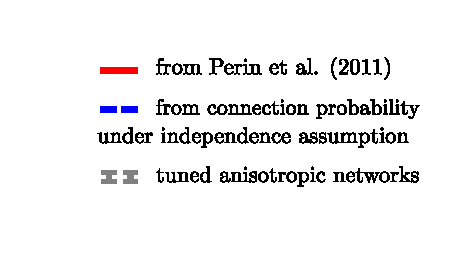
\includegraphics[width=0.5\textwidth]{%
      img/tuned_legend.pdf}   
  }%
  \vspace{-0.15cm}
  \caption{\textbf{Overrepresentation of reciprocal connections
      independent of } Comparison of occurrences of one- and
    bidirectionally connected neuron pairs in (gray) with profiles
    found by \textcite{Perin2011} (red), shows that overrepresentation of
    bidirectional pairs is distance-independent and not connected to
    anisotropy.  \textbf{A)} Overall connection probability in the
    adapted anisotropic networks was successfully tuned to reflect
    connection probability found by Perin et al. \textbf{B)-C)}
    Probabilities for a random neuron pair to display , 
    (\smtcite{875505b0})} %?? fix width issue!!
  \label{fig:perin_profiles_and_such}
\end{figure}



%%% Local Variables: 
%%% mode: latex
%%% TeX-master: "../dplths_document"
%%% End: 

 

\section{Motifs}

In this chapter we analyze the strucarl. The term motif referes
to... . Studies of \textcite{Song2005} and \textcite{Perin2011} show
stuff.

\subsection*{Three-neuron patterns}

Song motifs:


\begin{figure}[H]
  \centering
  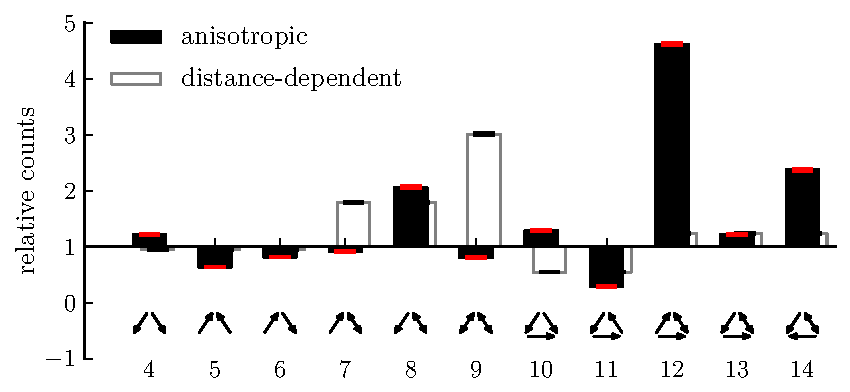
\includegraphics[width=0.95\linewidth]{%
    plots/4839ce41_aniso_dist.pdf} 
  \captionsetup{skip=8pt}
  \caption{\textbf{Relative occurrence of three-neuron patterns}
    Extracting the counts of three-node motifs in anisotropic (filled
    bars) and distance-dependent networks (unfilled bars), the
    quotient of the obtained count with the number of occurrences
    expected from the two-neuron connection probabilities in the
    networks (rs =, ,, cf.) shows the over- and underrepresentation of
    specific motifs in the network (red and black errorbars are
    SEM). In anisotropic networks pattern number \enquote{12}, for
    example, appears around five times more often than we would expect
    from the occurrence two-neuron connections. The relative counts
    for anisotropic networks resemble the findings of
    \textcite{Song2005} and differ significantly from the counts in
    distance-dependent networks, implying that anisotropy has a strong
    influence on the relative occurrence of three-neuron
    patterns. (\smtcite{4839ce41}) }
  \label{fig:distance_theory_compare}
\end{figure}




\begin{figure}[H]
  \centering
  \includegraphics[width=0.95\linewidth]{%
    plots/7c826e10_test.pdf} 
  \captionsetup{skip=8pt}
  \caption{\textbf{Relative occurrence of three-neuron patterns}
    Extracting the counts of three-node motifs in anisotropic (filled
    bars) and distance-adependent networks (unfilled bars), the
    quotient of the obtained count with the number of occurrences
    expected from the two-neuron onnection probabilities in the
    networks (rs =, ,, cfsdfg.) shows the over- and underrepresentation of
    specific motifs in the network (red and black errorbars are
    SEM). In anisotropic networks pattern number \enquote{12}, for
    example, appears around five times more often than we would expect
    from the occurrele the findings of
    \textcite{Song2005} and differ significantly from the counts in
    distance-dependent networks, implying that anisotropy has a strong
    influence on the relative occurrence of three-neuron
    patterns. (\smtcite{4839ce41}) }
  \label{fig:distance_theory_compare}
\end{figure}



\begin{figure}[H]
  \centering
  \renewcommand{\tabcolsep}{0pt}
  \setlength\extrarowheight{0pt}
  \begin{tabular}{ll}
    \begin{overpic}[width=0.5\textwidth]{%
        /users/hoffmann/research/cn_k_test.pdf}
      %\put(12,56){\small $\eta = 0$}
    \end{overpic}
    &
    \begin{overpic}[width=0.5\textwidth]{%
        /users/hoffmann/research/cn_k_test.pdf}
      %\put(12,56){\small $\eta = 0.25$}
    \end{overpic}
    \\
    \begin{overpic}[width=0.5\textwidth]{%
        /users/hoffmann/research/cn_k_test.pdf}
      %\put(12,56){\small $\eta = 0.5$}
    \end{overpic}
    &
    \begin{overpic}[width=0.5\textwidth]{%
        /users/hoffmann/research/cn_k_test.pdf}
      % \put(12,56){\small $\eta = 0.75$}
      %\put(4,-4){\small$0$}\put(78,-4){\small$200$}
    \end{overpic}
    \\
    % \begin{overpic}[width=0.28\textwidth]{%
    %     plots/77995b6b_in100.pdf}
    %   \put(12,56){\small $\eta = 1$}
    %   \put(4,-4){\small$0$}\put(78,-4){\small$200$}
    % \end{overpic}
    % & 
    % \begin{overpic}[width=0.28\textwidth]{%
    %     plots/77995b6b_indst.pdf}
    %   \put(12,56){\small distance}
    %   \put(4,-4){\small$0$}\put(78,-4){\small$200$}
    % \end{overpic}
    % \\
  \end{tabular}
  \caption{\textbf{In-degxree distrbution not affected by varying
      degrees of anisotropy} 
    (\smtcite{77995b6b}). }
  \label{fig:in_degree_rewiring}
\end{figure}



%%% Local Variables: 
%%% mode: latex
%%% TeX-master: "../dplths_document"
%%% End: 


\section{Common neighbor rule}


In their study, Perin et al.\ follow their report of increased
\marginpar{common neighbor rule as underlying principle?}  edge counts
in neuron clusters with the observation of a \enquote{common neighbor
  rule}\index{common neighbor rule}. Relying once again on their data
in the rat's somatsensory cortex, Perin et al.\ find that not only do
neuron pairs with a high number of common neighbor count appear
significantly more often than expected, but also that such pairs
display a higher probability of being connected. In fact, the
relationship between pair connectivity and number of common neighbors
appears to be linear. Perin et al.\ also report that this effect is
most pronounced when only considering common in-neighbors, that is
other neurons that are projecting to both neurons in the pair.

Here we also investigate our networks for the existence of such a
common neighbor relationship. Simultaneously recording connection
probabilities and the number of common neighbors between pairs of
neurons, we find inherent dependencies between the two quantities in
all network types (\autoref{fig:cm_rule}). 


\begin{figure}[H]
  \centering
  \makebox{%
    \begin{overpic}[width=0.5\textwidth]{%
         plots/5841710e_in.pdf}
      \put(21,56.6){\small\textbf{A}}
    \end{overpic}
    \hfill
    \begin{overpic}[width=0.5\textwidth]{%
        plots/5841710e_out.pdf}
      \put(21,56.6){\small\textbf{B}}
    \end{overpic}
  }%
  \vfill
  \vspace{0.11cm}
  \makebox{%
    \begin{overpic}[width=0.5\textwidth]{%
         plots/5841710e_all.pdf}
       \put(21,56.6){\small\textbf{C}}
    \end{overpic}
    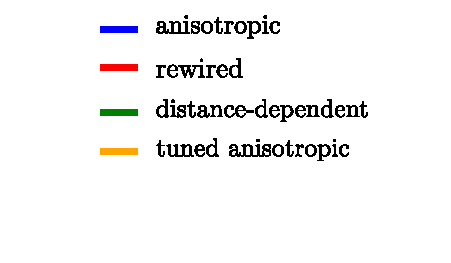
\includegraphics[width=0.5\textwidth]{%
      img/common_neighbor_legend.pdf}
  }
  \vfill
  \vspace{0.11cm}
  \makebox{%
    \begin{overpic}[width=0.5\textwidth]{%
         plots/5841710e_in_k.pdf}
      \put(20.5,57.5){\small\textbf{D}}
    \end{overpic}
    \hfill
    \begin{overpic}[width=0.5\textwidth]{%
        plots/5841710e_out_k.pdf}
      \put(20.5,57.5){\small\textbf{E}}
    \end{overpic}
  }%
  \captionsetup{skip=7pt}
  \caption{\textbf{Distance-independent overrepresentation of
      reciprocal connections}  (\smtcite{something})}
  \label{fig:cm_rule}
\end{figure}


Analyzing the results, we immediately note the sharp difference
between in- and out-neighbors in their effect on connection
probabilities in anisotropic networks, as well as in rewired
networks. Only in distance-dependent networks it appears that in- and
out-neighbors can be considered equivalent in their influence on
connection probabilities (\autoref{fig:cm_rule} A-B). Furthermore,
while the distribution of the number of common neighbors is consistent
in distance-dependent networks, the other network types display a
characteristic distribution of common out-neighbors
(\autoref{fig:cm_rule} D-E). This observation clearly relates to the
drastically different out-degree distributions in the different
networks found in
Section~\ref{sec:degree_distribution}. % Intertrepation: Connectivity
% in cortex asymmetric: synapse cortex
% and with Perin result in vs out

Both for in- and out-neighbors, we find characteristic curves
describing their influence on connection probabilities. The
in-neighbor profiles split into two categories: While networks with
anisotropy in connectivity (blue, orange) display a constant increase,
distance-dependent network types (red, green) \marginpar{anisotropy
  induces characteristic common neighbor rule} show a sigmoidal shared
input-connection probability curve (\autoref{fig:cm_rule} A).  We thus
find a strong influence of anisotropy on the shared input
relationship, inducing a common neighbor rule characteristically
different from isotropic, distance-depen\-dent networks.

Does this anisotropy-induced rule reflect the findings in cortical
networks?  Perin et al.\ report a linear common neighbor relationship,
finding a stronger effect when considering only in-neighbors. Imposing
the common neighbor rule on \textit{in silico} networks reflecting a
distance-dependency as determined \textit{in vivo}, Perin et al.\ were
then able to reproduce the observed overrepresentation of high edge
counts in neuron clusters, identifying the common neighbor effect as
an underlying connection principle inducing increased high edge counts
in clusters comparable to the profiles shown in
\autoref{fig:perin6to12}. Showing not only the presence of such an
edge count overrepresentation in anisotropic networks, but also
finding that only networks featuring anisotropy display an
approximately linear relationship between common inputs and connection
\marginpar{anisotropy as underlying connection principle!}
probability, we identify anisotropy in connectivity as a candidate for
an underlying connection principle motivated from neuronal morphology,
to induce a common neighbor rule, that may be at the heart of many of
the non-random connectivity statistics observed in local cortical
networks.

Extending the analysis of shared inputs in the different network
types, we further observe that anisotropy affects the number of common
in-neighbors typically observed itself (\autoref{fig:cm_rule} D). We
specifically find that increases anisotropy in connectivity induces an
increased variance in the distribution of common inputs of a random
neuron pair \autoref{fig:common_input_rew}). Such increased variance
may provide an important advantage in the processing of information,
allowing a heightened functional specificity in the network, where
many neurons do not share many common inputs, enabling a high variety
of functionality, and where few neuron pairs have a high number of
shared inputs, strengthening their correlation and thus their capacity
to relay related information.



\begin{figure}[H]
  \centering
  \makebox{%
    \begin{overpic}[width=0.493\textwidth]{%
        plots/5841710e_in_k_tanfitrew.pdf}
      \put(87.5,58.2){\small\textbf{A}}
    \end{overpic}
    \hfill
    \begin{overpic}[width=0.5\textwidth]{%
        plots/ffcefe9b.pdf}
      \put(89,58.2){\small\textbf{B}}
    \end{overpic}
  }%
  \captionsetup{skip=7pt}
  \caption{\textbf{Anisotropy increases variance of common input
      distribution} Recording common in-neighbor counts for random
    neuron pairs in tuned anisotropic networks and their rewired
    versions reveals increased variance in networks with a high degree
    of anisotropy. \textbf{A)} Common in-neighbor distribution for
    original tuned anisotropic networks ($\eta = 0$, blue) and rewired
    versions with $\nicefrac{1}{4}$ of all edges rewired ($\eta =
    0.25$, red) and completely rewired ($\eta =1 $, green).
    (\smtcite{5841710e}) \textbf{B)} Variance of the common
    in-neighbor distributions declines with increasing rewiring factor
    $\eta$; highest variance is found in networks with the highest
    degree of anisotropy ($\eta = 0$). Errorbars SEM. (\smtcite{ffcefe9b})}
  \label{fig:common_input_rew}
\end{figure}


%%% Local Variables: 
%%% mode: latex
%%% TeX-master: "../dplths_document"
%%% End: 



\section{Discussion}\label{sec:discussion}



In their study \textcite{Perin2011} were able to relate increased
edge-counts in neuron clusters to a \textit{common neighbor rule} - a
specific relationship between common in- or outputs in a neuron pair
and the probability for the pair to be connected - identifying an
underlying principle for the occurrence of non-random connectivity in
local circuits. Perin et al.\ suggest that (fire together wire
together). In this structural analysis we found non-random
connectivity resembling the findings of Song et al./ and , purely from
a g. Identifying a common neighbor rule as the inherent, that
non-random connectivity statistics might arrise from morphological
restrictions rather than plastic processes.



%%% Local Variables: 
%%% mode: latex
%%% TeX-master: "../dplths_document"
%%% End: 















%%% Local Variables: 
%%% mode: latex
%%% TeX-master: "../dplths_document"
%%% End: 
